\documentclass[a4paper,10pt]{article}
\usepackage[utf8]{inputenc}
\usepackage{amsmath,amssymb}
\usepackage{enumerate}
\usepackage{ngerman}
%\usepackage{graphicx}
\usepackage{ifpdf}
\usepackage[usenames]{color}
\usepackage[left=2.5cm,right=2.5cm,top=2.5cm,bottom=2.5cm]{geometry}
\usepackage[titles]{tocloft}
\usepackage[colorlinks=true,linkcolor=black]{hyperref}
\usepackage[pdftex]{graphicx}
\usepackage{geometry}
%\geometry{top=0cm,bottom=0cm,left=0cm,right=0cm,nohead,nofoot}


\title{Entwurf}
\date{}

\author{Usman Ghani Ahmed \\
Philip Caroli\\
Maximilian Madlung\\ 
Jeremias Mechler\\ 
Fabian Neundorf}

\ifpdf
\DeclareGraphicsExtensions{.pdf,.png}
\else
\DeclareGraphicsExtensions{.eps}
\fi

% Einrückung bei Absätzen
\setlength{\parindent}{0mm}
% Zeilenabstand bei Absätzen
\setlength{\parskip}{2mm}

\begin{document}
 
\vspace{5cm}
\maketitle
\begin{center}
\vspace{3cm}
\huge{Praxis der Softwareentwicklung \\
Gruppe 3 \\[0.5cm]
Entwicklung eines "`Monopoly"'-ähnlichen Spiels \\[0.5cm]
%
\includegraphics[height=2cm]{kitlogo_de_rgb}  \\[0.5cm]
WS 2010 / 2011} \\[2cm]
Version 1.1
%\textcolor{red}{! DRAFT !}
\end{center}

\newpage

\tableofcontents

\newpage

\section{Architektur}

%GEMEINSAME-SCHNITTSTELLE
\subsection{Gemeinsame Schnittstelle}
\subsubsection{Motivation}
Wir haben gemeinsam die Schnittstellen entsprechend unseren Bedürfnissen angepasst. Diese besteht einerseits aus den Interfaces "`IServer"', "`IServerTrade"', "`IServerAuction"' und "`IClient"', sowie aus der Klasse "`Rules"'.
\subsubsection{Schnittstellen}
\begin{itemize}
\item IServer \\
Die IServer-Schnittstelle dient als gemeinsame Basis für die Clients.

Methoden:
\begin{itemize}
\item int getPlayerPiecePosition(int playerID) \\
Gibt die aktuelle Position des Spielers mit der ID "`playerID"' zurück.
\item int addPlayer(IClient client) \\
Fügt einen Client hinzu.
\item void setPlayerReady(int player) \\
Setzt den Spieler mit der ID "`player"' auf bereit.
\item String getPlayerName(int player) \\
Gibt den Namen eines Spielers zurück.
\item int getPlayerColor(int player) \\
Gibt die Farbe des Spielers zurück.
\item Rules getRules() \\
Gibt den Regelsatz zurück.
\item String getEstateName(int position) \\
Gibt den Namen des Grundstücks auf der in "`position"' definierten Position zurück.
\item int getEstateColorGroup(int position) \\
Gibt die Farbgruppe des Grundstückes zurück. Nicht-negative Werte stehen dabei für die eigentlichen Farbgruppen in der Reihenfolge auf dem Brett. Negative Werte stehen für Sonderfelder:
\begin{description}
\item[-1] Startfeld
\item[-2] Gefängnis
\item[-3] Frei parken
\item[-4] "`gehe in das Gefängnis"'
\item[-5] Ereignisfelder
\item[-6] Gemeinschaftsfelder
\item[-7] Bahnhöfe
\item[-8] Infrastrukturgebäude
\item[-9] Sondersteuerfelder
\end{description}
Weitere sind benutzerdefiniert.
\item int getEstateHouses(int position) \\
Liefert die Zahl der gebauten Häuser an der gegebenen Position. Ein Hotel wird dabei als die Zahl 5 repräsentiert.
\item int getEstatePrice(int position) \\
Liefert den Kaufpreis des Grundstücks an der gegebeben Position.
\item int getEstateRent(int position, int houses) \\
Liefert die Höhe der Miete für ein Grundstück in der angegebenen Bebauung. Dabei kann das Grundstück sowie die Bebauung gewählt werden.
\item String getGameStatusMessage(int playerID) \\
Liefert die aktuelle Spielmeldung für einen Spieler. Dies können entweder reine Statusmeldungen
oder für den Spielfluss entscheidende Fragen an den Spieler sein, z.B. ob man die Geldstrafe im Gefängnis zahlt oder etwa ob
man ein Grundstück erwerben möchte. In den letzteren Fällen muss dem Server zunächst mit "`accept()"' oder "`decline()"'
geantwortet werden bevor andere Aktionen (z.B. Häuser bauen, Zug beenden) getätigt werden.
\item boolean isMortgaged(int position) \\
Gibt an, ob das gegebene Grundstück mit einer Hypothek belastet ist.
\item int getOwner(int position) \\
Gibt den Eigentümer des Grundstücks an der gegebenen Position an. Falls das Grundstück der Bank gehört, ist das Ergebnis -1.
\item int getDiceValue() \\
Liefert die aktuelle Augensumme.
\item int[] getDiceValues() \\
Liefert die Werte der einzelnen Würfel.
\item int getPlayerCash(int playerID) \\
Liefert das aktuelle Barvermögen eines Spielers. Ein negativer Wert bedeutet dabei, dass der Spieler bankrott ist und aus dem Spiel ausgeschieden ist.
\item int getPlayerOnTurn() \\
Liefert die ID des Spielers, der momentan am Zug ist. Falls das Spiel
momentan nicht läuft, ist das Ergebnis -1.
\item int getNumberOfGetOutOfJailCards(int playerID) \\
Liefert die Zahl der "`Du kommst aus dem Gefängnis frei"'-Karten eines Spielers.
\item int getNumberOfHousesLeft() \\
Liefert die Zahl der noch in der Bank vorhandenen Häuser.
\item int getNumberOfHotelsLeft() \\
Liefert die Zahl der noch in der Bank verbliebenen Hotels.
\item boolean rollDice(int playerID) \\
Rollt die Würfel und bewegt die Figur (falls sie nicht im Gefängnis ist).
Falls dem Spieler eine für den Spielfluss entscheidende Frage gestellt wird, so muss diese
danach mit "`accept()"' oder "`decline()"' beantwortet
werden. Es kann nur einmal am Anfang des Zuges gewürfelt werden (bzw. dreimal im Gefängnis).
\item boolean accept(int playerID) \\
Gibt eine positive Antwort auf eine spielentscheidende Frage des Servers.
Kann nur getätigt werden, wenn die aktuelle Statusmeldung eine solche
Frage ist.
\item boolean decline(int playerID) \\
Gibt eine negative Antwort auf eine spielentscheidende Frage des Servers.
Kann nur getätigt werden, wenn die aktuelle Statusmeldung eine solche
Frage ist.
\item boolean endTurn(int playerID) \\
Beendet den aktuellen Zug. Kann nur getätigt werden, wenn gewürfelt und
alle spielentscheidenen Fragen beantwortet wurden.
\item boolean declareBankruptcy(int playerID) \\
Erklärt Bankrott. Setzt das Barvermögen des jeweiligen Spielers auf einen negativen Wert.
\item boolean construct(int playerID, int position) \\
Baut "`ein"' Haus auf das angegebene Grundstück. Kann nur getätigt
werden, wenn die Bedingungen dafür erfüllt sind.
\item boolean deconstruct(int playerID, int position)
Löst "`ein"' Haus auf dem angegebenen Grundstück auf. Kann nur
getätigt werden, wenn die Bedingungen dafür erfüllt sind.
\item boolean toggleMortgage(int playerID, int position)
Nimmt eine Hypothek auf das angegebene Grundstück auf oder zahlt diese
zurück.
\item void sendMessage(String text)
Sendet eine öffentliche Nachricht an alle.
\item void sendPrivateMessage(String text, int reciever)
Sendet eine private Nachricht an den entsprechenden Empfänger.
\end{itemize}
%IServerTrade

\item IServerTrade \\
Eine Erweiterung der IServer-Schnittstelle, sodass auch Auktionen abgewickelt werden k"onnen

Methoden:
\begin{itemize}
\item int getAuctionState()
Gibt den derzeitigen Stand der Auktion an
\begin{description}
\item[-1] keine Auktion l"auft
\item[0] Auktion l"auft
\item[1] "`Zum Ersten"'
\item[2] "`Zum Zweiten"'
\item[3] Auktion abgeschlossen, Daten sind noch abrufbar
\end{description}
\item int getAuctionedEstate()
Gibt die Position des Grundst"ucks zur"uck, das versteigert wird
\item int getHighestBid()
Gibt das bisher h"ochste Gebot zur"uck
\item int getHighestBidder()
Gibt den bisher h"ochsten Bieter zur"uck
\item boolean placeBid(int playerID, int amount)
Gibt ein Gebot in der H"ohe amount des Spielers playerID ab
\end{itemize}
\item IServerAuction \\
Erweiterung der Schnittstelle IServer, sodass gehandelt werden kann

Methoden:
\begin{itemize}
\item boolean initTrade(int actingPlayer, int partnerPlayer)
Startet einen Handel zwischen actingPlayer und partnerPlayer
\item int getTradeState()
Gibt den Zustand des Handels an
\begin{description}
\item[-1] Dezeit kein Handel
\item[0] Handelssitzung l"auft, bisher noch kein Angebot
\item[1]Handelssitzung l"auft, Angebot liegt vor, noch keine Entscheidung
\item[2] Handelsangebot wurde abgewiesen
\item[3] Handelsangebot wurde angenommen
\end{description}
\item int getPartner()
Liefert den Handelspartner
\item boolean offerCash(int playerID, int cash)
Bietet Geld
\item offerGetOutOfJailCard(int playerID)
Bietet eine "`Komme aus dem Gef"angnis frei Karte"' an
\item boolean offerEstate(int playerID, int position)
Bietet ein Grundst"uck an
\item boolean requireCash(int playerID, int position)
Fordert Geld
\item boolean requireGetOutOfJailCard(int playerID)
Fordert eine "`Komme aus dem Gef"angnis frei Karte"'
\item requireEstate(int playerID, int position)
Fordert ein Grundst"uck
\item int[] getOfferedEstates
Liefert alle angebotenen Grundst"ucke
\item int getOfferedCash()
Liefert das angebotene Geld
\item getNumberOfOfferedGetOutOfJailCards()
Liefert die Anzahl angebotener "`Komme aus dem Gef"angnis frei"'-Karten
\item int[] getRequiredEstates()
Liefert alle angeforderten Grundst"ucke
\item int getRequiredCash()
Liefert das geforderte Geld
\item int getNumberOfRequiredGetOutOfJailCards()
Liefert die Anzahl geforderter "`Komme aus dem Gef"angnis frei"'-Karten
\item boolean cancelTrade(int playerID)
Bricht die aktuelle Handelssitzung ab
\item boolean proposeTrade(int playerID)
Schl"agt einen Handel vor, zuvor wurde mit \textit{offer/require Estate/Cash/GetOutOfJailCard} festgelegt, um was gehandelt wurde
\end{itemize}
\item IClient \\
Wurde gemeinsam mit der anderen Gruppe entwickelt. Dieses Interface dient dazu, die Kommunikation von Serverseite aus zu den Clienten zu erm"oglichen

Methoden:
\begin{itemize}
\item string getName()
Liefert den Namen des Spielers
\item string getLanguage()
Gibt die Sprache des Spielers zur"uck, zB ""de"" f"ur deutsch, ""fr"" f"ur Franz"osisch
\item informStartGame(int numberOfPlayers)
Informiert den Clienten, dass das Spiel beginnt
\item void informTurn()
Informiert den Clienten, dass er an der Reihe ist
\item void informDiceValues(int[] diceValues, int playerID)
Informiert den Clienten, dass ein neuer W"urfelwurf vorliegt
\item void informCashChange(int playerID, int cashChange)
Informiert den Clienten, dass sich ein Kontostand ge"andert hat
\item void informStreetBuy(int playerID)
Informiert den Clienten, dass ein Spieler eine Stra"se gekauft hat
\item void informConstruct(int position)
Informiert den Clienten, dass eine Stra"se ausgebaut wurde
\item void informDestruct(int position)
Informiert den Clienten, dass eine Stra"se um einen Rang verringert wurde
\item void informMortageToogle(int position)
Informiert den Clienten, dass eine Hypothek aufgenommen/abbezahlt wurde
\item void informCardPull(String text, boolean communityCard)
Informiert den Clienten, dass er eine Gemeinschafts- oder Ereigniskarte gezogen hat
\item void informBankruptcy()
Informiert den Clienten, dass der aktuelle Spieler bankrott ist
\item void informMessage(string text, int sender, boolean privateMessage)
Informiert den Clienten, dass er eine neue Nachricht empfangen hat
\end{itemize}
\end{itemize} % SCHNITTSTELLEN

\subsubsection{Klassen}
\begin{itemize}
\item Rules \\
Diese Klasse beschreibt einige Grundregeln. Die Eigenschaften sind dabei als öffentliche geschützte Attribute verfügbar.

Attribute:
\begin{itemize}
\item public final int startMoney \\
Dieser Wert gibt das verfügbare Startgeld an.
\item public final int goMoney; \\
In diesem Wert steht, wie viel Geld man bekommen, sobald man über Los kommt.
\item public final boolean doubleMoneyOnGo \\
Dieser Wahrheitswert ist wahr, wenn der Spieler doppelt so viel Geld bekommen soll, wenn er auf den Los-Feld zum stehen kommt.
\item public final boolean tradesWithMoney \\
Über diesen Wert kann bestimmt werden, ob beim Handeln die "`Ware"' Geld mitbenutzt werden darf.
\item public final boolean auctionActive \\
Hiermit kann man Auktionen aktivieren oder deaktivieren.
\item public final boolean moneyOnFreeParking;
Sofern dieser Wert auf wahr steht, bekommt der Spieler das Geld aus den Steuertopf sobald dieser auf das Feld "`Frei parken"' kommt.
\end{itemize}

Methoden:
\begin{itemize}
\item public Rules(int startMoney, int goMoney, boolean doubleMoneyOnGo, boolean tradesWithMoney, boolean auctionActive, boolean moneyOnFreeParking) \\
Dieser Konstruktor kann einmal die Spielregeln setzen.
\item public Rules() \\
Dieser setzt die Spielregeln auf die Standardregeln von Monopoly:
\begin{enumerate}
\item 30.000 Startgeld
\item 4.000 Geld bei Los
\item kein doppeltes Geld, wenn man auf Los zieht
\item Geld ist beim Handeln erlaubt
\item Auktionen sind erlaubt
\item Man erhält kein Geld aus den Steuertopf, wenn man auf das "`Frei parken"'-Feld kommt.
\end{enumerate}
\end{itemize}
\end{itemize} % KLASSEN

%CLIENT-GRUNDGERUEST
\subsection{Client-Grundgerüst}
Das Client-Grundgerüst dient als Grundgerüst für den KI- und GUI-Client.
\subsubsection{Klassen}
\begin{itemize}
\item ClientBase\\
Ist diejenige Klasse, die von den Clients vererbt wird. Diese Klasse ist abstrakt, da die Methoden aus "`IClient"' nicht in dieser Klasse implementiert werden.

Verwendet:
\begin{itemize}
\item IClient
\end{itemize}
Attribute:
\begin{itemize}
\item private IServer server \\
Die entsprechende Serverinstanz wird hier abgelegt. Dabei handelt es sich u.U. um das Netzwerk.
\item protected GameLogic gameLogic \\
Ist eine Referenz auf das aktuelle Spielfeld und den Spielregeln.
\end{itemize}
Methoden:

\begin{itemize}
\item protected void connect(string host, int port) \\
Verbindet sich mit einem Server mithilfe eines Hosts und den entsprechenden Port.
\item protected void connect(IServer server) \\
Setzt einen vorhanden IServer als entsprechendes Server-Objekt.
\item Folgende Methoden werden für den IServer gewrappt. Dies geschieht um vorher zu testen, ob das Regelwerk den Zug erlaubt.
\begin{itemize}
\item protected void accept()
\item protected void decline()
\item protected void rollDice()
\item protected void endTurn()
\item protected void declareBankruptcy()
\item protected void construct(int street)
\item protected void destruct(int street)
\item protected void toggleMortgage(int street)
\item protected void sendMessage(string text)
\item protected void sendPrivateMessage(string reciever, string text)
\end{itemize}
\end{itemize} % Methoden
\end{itemize} % Klassen

%KI-CLIENT
\subsection{KI-Client}
\subsubsection{Interfaces}
\begin{itemize}
\item ValuationFunction

Das Interface "`ValuationFunction"' dient zur Beschreibung der Bewertungsfunktionen, die aus dem Paper von Frayn übernommen wurden. Das Interface stellt allen Funktionen jeweils eine Instanz der Spielregeln und des Spielzustands zur Verfügung. Durch diese können die Bewertungsfunktionen auf alle Informationen zugreifen.
Die statische und öffentliche Methode "`returnValuation"', die von den implementierenden Klassen bereitgestellt wird, gibt die Bewertung des möglichen Spielzugs als Gleitkommaahl zurück. Die Bewertungsfunktionen sind \textit{Singletons}.
\item Command

Zur Ausführung des am besten bewerteten Spielzugs wird das Entwurfsmuster "`Befehl"' verwendet. Das Interface "`Command"' stellt das Grundgerüst für die Befehle dar.
\end{itemize}
\subsubsection{Klassen}
\begin{itemize}
\item AiClient

Diese Klasse erbt vom Client-Grundgerüst und implementiert die dort vorgegebenen (abstrakten) Methoden.
\item Valuator

Diese Klasse bewertet die möglichen Spielzüge, die in dieser Klasse auch bestimmt werden. Der Spielzug mit der besten Bewertung wird an \textit{AiClient} als Befehls-Objekt zurückgegeben und dort ausgeführt.
In der Klassenvariable "`weights"' sind die einzelnen, noch zu bestimmenden Gewichte der einzelnen Bewertungsfunktionen gespeichert, die zusammen die Gesamtbewertung ergeben.
\item ValuationParameters

In der Klasse "`ValuationParameters"' werden die von den Bewertungsfunktionen benötigten und noch zu bestimmenden Gewichte gespeichert. Diese sind zur Laufzeit nicht veränderbar.
\item PropertyValuator

Dient zur Bewertung eines kaufbaren Objekts, z.B. einer Straße
\item PropertyGroupValuator

Dient zum Bewerten von Objektgruppen, insbesondere also aller Straßen gleicher Farbe
\item BuildingOnPropertyValuator

Bewertet das Bauen von Häusern, Hotels, etc.
\item PrisonValuator

Befindet sich der KI-Client im Gefängnis, entscheidet diese Klasse, ob Freikaufen rentabel ist.
\item MortgageValuator

Dient zum Bewerten von Hypotheken.
\item CapitalValuator

Es ist laut Paper empfehlenswert, immer eine Mindestmenge Geld zu besitzen.
\item OutOfPrisonCommand

Sofern es sinnvoll ist, sich aus dem Gefängnis freizukaufen, wird eine Instanz dieser Klasse zurückgegeben
\item BuyPropertyCommand

Soll eine Straße etc. gekauft werden, wird dies von diesem Befehl übernommen.

\item DeclineCommand

Soll die Spielmöglichkeit nicht durchgeführt werden, wird ein \textit{DeclineCommand}-Objekt zurückgegeben

\item MortgageCommand

Dient zum Aufnehmen von Hypotheken

\item AuctionCommand

Dient zum Starten und Teilnehmen an einer Auktion

\item TradeCommand

Siehe Unterklassen

\item RequestTradeCommand

Nimmt einen Handel mit Spieler \textit{remotePlayer} entweder um Geld, eine Gefängnisfreikarte oder eine Straße auf.

\item OfferTradeCommand

Bietet bei einem bereits inittiertem Handel dem Spieler \textit{remotePlayer} entweder Geld, eine Gefängnisfreikarte oder eine Straße.
\end{itemize}


%GUI-CLIENT
\subsection{GUI-Client}

%Beschreibung
Der GUI-Client baut auf dem Clientgrundger"ust auf bietet eine graphische Oberfl"ache, um dessen Zustand anzuzeigen und darüber den Server aufzurufen.

\subsubsection{Klassen}

\begin{itemize}
%GameFieldPieceCollection
\item GameFieldPieceCollection\\
%end GameFieldPieceCollection

%GameFieldPiece
\item GameFieldPiece\\
Ist ein einzelnes Feld auf den Spielbrett.

Methoden:
\begin{itemize}
\item GameFieldPiece(int cardId, String name, int position, Image image)
Erstellt ein neues Feld auf den Spielbrett.
\end{itemize}
%end GameFieldPiece

%GameFieldCard
\item GameFieldCard \\
Ist ein kaufbares Feld.

Verwendet:
\begin{itemize}
\item GameFieldPiece
\end{itemize}

Methoden:
\begin{itemize}
\item void turnAround() \\
Dreht ein Feld um.
\item void switchOwner(int player) \\
Setzt den Besitzer auf die neue ID.
\end{itemize}
%end GameFieldCard

%InteraktionsPopup
\item InteractionPopup \\
Ein graphisches Fenster zum Anzeigen diverser Interaktionsmöglichkeiten.

Attribute:
\begin{itemize}
\item string message
\item boolean acceptEnabled
\item boolean declineEnabled
\item boolean isActive
\end{itemize}

Methoden:
\begin{itemize}
\item void clear() 
\\Löscht die Nachricht und zeigt nichts an.
\item void showMessage(string Message, boolean accepting, boolean declining)
\\Zeigt eine neue Nachricht an, je nachdem sind "`accept"' und "`decline"' aktiviert.
\item void showInformation(string message)
\\Zeigt eine einfache Nachricht ohne Auswahlmöglichkeit an.
\end{itemize}
%end InteractionPopup

%Chatfenster
\item ChatWindow\\
Eine graphische Komponente, die ein Chatfenster, bestehend aus einem (scrollbaren) Anzeigefenster und einem Texteingabefenster besteht. Bei Empfang einer Nachricht wird diese im Anzeigefenster ausgegeben. Es können mehrere Nachrichten gleichzeitig angezeigt werden und neue Nachrichten werden unter alten Nachrichten geschrieben. Bei Eingabe einer Nachricht in das Texteingabefenster wird die Nachricht an den Server geschickt

Methoden:
\begin{itemize}
\item void clear()
\\ l"oscht alle Nachrichten
\item void write(ChatMessage message)
\\F"ugt der Liste eine neue Nachricht hinzu
\end{itemize}
%end Chatfenster

%ChatMessage
\item ChatMessage \\
Beinhaltet alle Elemente einer Chat-Nachricht.

Attribute:
\begin{itemize}
\item Player sender
\\Der Spieler, von dem diese Nachricht gesendet wurde.
\item string message
\\Der Text der Nachricht.
\item DateTime date
\\Wann die Nachricht empfangen wurde.
\end{itemize}

%PlayerInfoField
\item PlayerInfoField\\

Eine graphische Komponente, die wesentliche Informationen über einen Spieler anzeigt und muss bei Veränderungen des Spielerstatus die neuen Daten anzeigen.

Attribute:
\begin{itemize}
\item int player \\
Ist der Spieler des Infofeldes.
\end{itemize}

Methoden:
\begin{itemize}
\item PlayerInfoField(int player) \\
Initialisiert ein Eintrag mit den gegebenen Spieler.
\item void switchStatus() \\
Ändert den Zustand des Spielers zwischen \textit{wartend} und \textit{spielend}.
\end{itemize}
%end PlayerInfoField

%PlayerInfoWindow
\item PlayerInfoWindow \\
Verwaltet alle einzelnen \textit{PlayerInfoField}-Einträge.

Methoden:
\begin{itemize}
\item void turnOn(int player)
\\Setzt den Spieler auf \textit{spielend}.
\item void changeCash(int player, int newCashValue)
\\Setzt den neuen Bargeld-Wert.
\end{itemize}

\item Card \\
Eine Ereignis-/Gemeinschaftskarte.

Methoden:
\begin{itemize}
\item void turnAround() \\
Deckt diese Karte auf.
\end{itemize}

\item CardStack\\
Ein einzelner Kartenstapel.

Methoden:
\begin{itemize}
\item void addCard(int cardId) \\
Fügt eine Karte diesen Kartenstapel hinzu.
\item void removeCard(int cardId) \\
Entfernt eine Karte.
\end{itemize}

\item CardWindow \\
Verwaltet die Kartenstapel.

Methoden:
\begin{itemize}
\item void addCard(int cardStack, int cardId) \\
Fügt eine Karte einen Kartenstapel hinzu.
\item void removeCard(int cardId) \\
Entfernt eine Karte.
\end{itemize}

\item GUISettings \\
Verwaltet die GUI-Einstellungen.

Attribute:
\begin{itemize}
\item int width \\
Die Breite des Fensters.
\item int height \\
Die Höhe des Fensters.
\item String lastIP \\
Die letzte IP.
\item String playerName \\
Der Spielername.
\end{itemize}
\end{itemize}

%LOGIKREGELNZUSTAND
\subsection{Logik, Regeln, Zustand}

%Beschreibung
Dieses Paket enthält den Zustand, sowie die Regeln und die Logik um Eingaben zu validieren, Informationen zu erlangen oder einzufügen.


%GameLogic
\begin{itemize}
\item GameLogic \\
Beinhaltet den Inhalt des Pakets und ist die Kontaktstelle nach außen.

Methoden:
\begin{itemize}
\item boolean newGame()
\\Startet ein neues Spiel, lädt die Regeln und erstellt einen Zustand.
\item boolean addPlayer(int playerId, String playerName, int playerCash)
\\Fügt dem Spiel einen Spieler hinzu und gibt an ob es geklappt hat, schließlich dürfen laut Monopolyregeln z.B. nur maximal 8 Spieler spielen.
\item void addMessage(int messageId, int playerId, String text)
\\Fügt dem Chat eine Nachricht hinzu.
\item void addRoll(int player, int[] dices)
\\Fügt einen neuen Wurf dem Status hinzu
\item void startGame()
\\Startet das Spiel (Also aus der GUI aus gesehen vom Warteraum aufs Spielbrett)
\item void movePlayer(int player, int street)
\\Bewegt einen Spieler zu einer Straße
\item void buyStreet(int player, int street)
\\Gibt dem Spieler eine Straße
\item void upgradeStreet(int player, int street, int level)
\\Setzt eine Straße auf ein neues Level
\item void useCard(int player, int card)
\\Benutzt für den Spieler eine Karte
\item void exitJail(int player)
\\Befreit den Spieler aus dem Gefängnis :)
\item GameState getGameState()
\\Setzt einen neuen Spielstatus

\end{itemize} % end methoden
%end GameState

%GameRules
\item GameRules \\
Beinhaltet die Regeln des Spiels.

Methoden:
\begin{itemize}
\item void setGameState(GameState gameState)
\\Setzt den Gamestate
\item boolean movementValid(int player, int field)
\\Ist der Spielzug ok?
\item boolean buyingValid(int player, int street)
\\Ist dieser Kauf ok?
\item boolean cardValid(int player, int card)
\\Ist das Verwenden der Karte von diesem Spieler ok?
\item boolean upgradeValid(int player, int street, int level)
\\Ist das Upgraden dieser Straße ok?
\item boolean playerHasCash(int player, int cash)
\\hat der Spieler das gewollte Geld?
\end{itemize} % end methoden
%end GameRules
\end{itemize} % end klassen

%SPIELSTATUS
\subsection{Spielstatus}


%Beschreibung
Alle Elemente, die den derzeitigen Zustand des Spiels beschreiben (z.B. Geldst"ande, teilnehmende Spieler) werden im Spielstatus gespeichert. Sowohl der Server als auch der Client besitzen einen Spielstatus.

\subsubsection{Klassen}

\begin{itemize}

%Spielzustand
\item GameState\\
Bietet Objekt-Zugriff auf alle Karten, Felder, Spieler, den Chat und bietet die Möglichkeit, Spielstände zu laden und zu speichern.

Methoden:
\begin{itemize}
\item getPlayer()

Gibt eine Menge mit Referenzen auf alle Spieler zurück
\item GameField getField()

Gibt eine Referenz auf das Spielfeld zurück
\item getCard()

Gibt eine Menge mit Referenzen auf alle Karten zurück
\item Chat getChat()

Gibt eine Referenz auf das Chat-Objekt zurück
\item boolean loadGameState(String path)

Lädt den unter \textit{path} abgelegten Spielstand. Ist das Laden erfolgreich, wird \textit{true} zurückgegeben, sonst \textit{false}
\item boolean saveGameState(String path)

Speichert den Spielstand nach \textit{path}. Ist das Speichern erfolgreich, wird \textit{true} zurückgegeben, sonst \textit{false}
\end{itemize} % end methoden
%end GameState

%Player
\item Player \\
Beschreibt einen Spieler aus Sicht des Spielstands

Attribute:
\begin{itemize}
\item int id

Die eindeutige Spieler-ID
\item Color color

Die Farbe des Spielers
\item String name

Der Name des Spielers
\item int possition

Die aktuelle Position des Spielers
\item int cash

Der aktuelle Geldbetrag des Spielers
\item int getOutOfJailCardsCount

Die Anzahl der "`Gehe aus dem Gefängnis"'-Karten des Spielers
\end{itemize} % end attribute

Methoden:
\begin{itemize}
\item Spieler(int id, int cash, String name)

Konstruktur. Für die Argumente siehe \textit{Attribute}
\item void addCash(int cash)

Fügt dem Spieler den Geldbetrag \textit{cash} hinzu.
\end{itemize} % end methoden
%end Player

%Feld
\item GameField \\
Dies Klasse beschreibt ein Spielfeld in Monopoly.

Attribute:
\begin{itemize}
\item int id

Eindeutige ID des Spielfeldes
\item int owner

ID des Players, der das Feld besitzt. Ist die ID $\le 0$, so gehört das Feld der Bank.
\item boolean turnedAround

Gibt an, ob eine Hypothek auf dem Feld ist.
\end{itemize} %end attribute

Methoden:
\begin{itemize}
\item void buy(int player)

Setzt \textit{owner} auf \textit{player}
\item void turnAround()

Setzt oder löscht eine Hypothek
\item boolean isTurnedAround()

Gibt zurück, ob eine Hypothek auf dem Feld ist
\end{itemize} % end methoden
%end Feld

%Straße
\item Street \\
Die Klasse Street beschreibt ein besitzbares Feld in Monopoly.

Verwendet:
\begin{itemize}
\item GameField
\end{itemize}

Attribute:
\begin{itemize}
\item int buildLevel

Gibt die aktuelle Ausbaustufe an
\end{itemize} %end attribute

Methoden:
\begin{itemize}
\item void upgrade(int level);

Erhöht die Ausbaustufe auf \textit{level}
\end{itemize} %end methoden
%Street end

%chat
\item Chat \\
Dient zum Versenden von Nachrichten an alle Spieler.

Methoden:
\begin{itemize}
\item void addMessage(int player, String message)

Gibt die Nachricht \textit{message} des Spielers \textit{player} weiter.
\end{itemize}
%end chat

%card
\item Card \\
Klasse der Karten

Attribute:
\begin{itemize}
\item int id

Eindeutige ID der Karte
\item int owner

ID des Eigentümers der Karte
\end{itemize}
%end Card
\end{itemize}
%end gamestate


%SPIELREGELN
\subsection{Spielregeln}


%Beschreibung
Die Regeln des Spiels

\subsubsection{Klassen}

\begin{itemize}
%CardRule
\item CardRule \\
Beinhaltet die Karten und ihre Regeln, sowie die Eigenschaften welche für diese Karte unabhängig vom Spielstatus sind.

Methoden:
\begin{itemize}
\item int getId()
\\Die Id der Karte
\item string getName()
\\der Name der Karte
\item Image getImage()
\\das Bild der Karte
\item void execute(int player)
\\Führt die Aktion dieser Karte aus
\end{itemize} %end methoden
%end CardRule

%CardAction
\item CardAction \\
Kapselung einer Aktion, die beim Ausspielen einer Ereignis- oder Gemeinschaftskarte ausgeführt werden kann.

Methoden:
\begin{itemize}
\item void execute(int player,int[] argument)
\\Diese Aktion wird von einer Karte mit dieser Regel ausgeführt
\end{itemize} %end methoden
%end CardAction

%FieldRule
\item FieldRule\\
Beinhaltet die Straßeninformationen die nicht durch den Spielstatus verändert werden.

Methoden:
\begin{itemize}
\item int getId()
\\Die Id des Feldes
\item String getName()
\\Der Name des Feldes
\item int getPosition()
\\Die Position des Feldes
\item Color getColor()
\\Die Farbe der Stra"sengruppe (optisch) und damit auch die Zuordnung zu einer Gruppe
\item int getPrice()
\\Die Kosten des Feldes
\item int getLevelPayment(int level)
\\Die Mietkosten je nach Gebäudelevel
\item Image getImage()
\\Das Bild des Feldes
\item void execute(int player)
\\Die Aktion wenn eine Spieler auf diesem Feld landet
\item void passTrough(int player)
\\Die Aktion wenn eine Spieler über dieses Feld marschiert oder auf ihm landet
\end{itemize} %end methoden
%end fieldrule
\end{itemize} % end SPIELREGELN

%SERVER
\subsection{Server}

%Beschreibung
Der Server verbindet mehrere Clienten in einem Spiel. Er ist die zentrale Stelle und dafür zuständig Spielzustandsänderungen durch Aufrufe des Clienten an den Server zu registrieren und darauf zu reagieren. Der Server implementiert die Schnittstellen IServer, IServerAuction und IServerTrade. Clienten können entweder direkt vom Server aus gestartet werden, oder "uber das Netzwerk Kontakt aufnehmen. In beiden F"allen passieren die meisten Interaktionen "uber IServer.

\subsubsection{Klassen}
\begin{itemize}
\item OjimServer \\
Dieser Server implementiert die Schnittstellen IServer, IServerTrade und IServerAuction. Er behandelt alle Spielstatusänderungen und Clients können sowohl direkt als auch über das Netzwerk angeschlossen werden. Der Server benutzt dabei eine Kommandozeilenschnittstelle.

Attribute:
\begin{itemize}
\item Ruleset ruleset
\item GameState gamestate
\item Network network
\end{itemize}

Methoden:
\begin{itemize}
\item boolean startGame(int playerCount) 
\item boolean loadGame(string path)
\item storeGame(int path)
\item loadSettings(int path)
\\l"adt die serverseitigen Einstellungen, z.B. welches Ruleset verwendet werden soll
\item boolean stopGame()
\\beendet das Spiel, speichert den Spielstand und trennt die Clienten
\item boolean startAIGames(int clientCount, int loops, string path)
\\Startet mehrere aufeinanderfolgende Spiele mit mehreren KI-Clienten. Das Ergebnis wird als Datei gespeichert
\end{itemize} % end methoden
\end{itemize} % end klassen

\subsection{Netzwerk}
Das Netzwerk stellt die Verbindung zwischen dem Client und dem Server dar, dabei ist es m"oglich das sich die Spieler in einem lokalen
Netzwerk befinden als auch "uber das Internet in einer anderen Java Virtual Machine arbeiten und am Spiel teilnehmen. Damit der Client Anfragen an den Server schicken kann, die die Ausf"uhrung von Methoden und die R"uckgabe von Ergebnissen beinhalten, verwenden wir den RMI (Remote Method Invocation)-Mechanismus , der uns das entfernte Aufrufen von Methoden erlaubt. Die Verbindung von Client und Server wird durch Stellvertreterobjekte(engl. \textit{proxies}) realisiert. Auf Seite des Clients wird ein Stellvertreter (\textit{Stub}) des entfernten Objekts (Skeleton) erzeugt, welcher die Daten die "ubermittelt werden kapselt und diese in Form von Nachrichten an den Server "ubermittelt. Die Daten beinhalten unteranderem die zu ausf"uhrende Methode inklusive R"uckgabetyp und alle Parameter. Durch den RMI-Compiler ist es m"oglich, die ben"otigten Stubs und Skeletons zu erzeugen. Damit von au"sen keine unberechtigten Zugriffe auf den Server erfolgen, werden Regeln in einer lokal zug"anglichen Datei erstellt und vom RMI Security Manager verwaltet.    
  
\subsubsection{Interfaces}
\begin{itemize}
\item NetOjim \\
Diese Schnittstelle erweitert die \textit{IServer}-Schnittstelle. Hier werden alle Methoden zur Verf"ugung gestellt, die das Server-Objekt auf Seite des Clients aufrufen kann
\end{itemize}

\subsubsection{Klassen}
\begin{itemize}
\item UnicastRemoteObject \\
Diese Klasse registriert das zu fernaufrufende Objekt bei der RMI-Verwaltung und verwaltet die "Ubertragung des zu fernaufrufenden Objekts zur Java Virtual Machine des Clients.
\item ImplBuffer \\
Diese Klasse erweitert die Klasse UnicastRemoteObject und implementiert das Interface IServer sowie das Interface \textit{Serializable}. Um das komplette Objekt als Parameter f"ur die RMI-Aufrufe zu "ubertragen, benutzen wir Object Serialization 
\item BufferServer \\
Diese Klasse Verwaltet das Remote-Objekt das f"ur den Client bereit steht.

Methoden:
\begin{itemize}
\item createBufferServer()
\\Meldet das Remote Objekt bei der RMI-Registry an und sorgt daf"ur das dieses "uber das Netzwerk unter einen bestimmten Namen ansprechbar ist
\end{itemize}

\item Socket \\
Stellt die Steckverbindung zum Netzwerk f"ur den Clienten dar
\item ServerSocket\\
Stellt die Steckverbindung zum Netzwerk f"ur den Server dar
\item Network\\
Verwaltet das Netzwerk.

Attribute:
\begin{itemize}
\item ServerSocket server
\item Socket client
\item List $<$ClientDetails$>$ client
\end{itemize}

Methoden:
\begin{itemize}
\item Network(ServerSocket server,Socket client, ServerDetails details) 
\item boolean waitingForClients()
\\Wartet bis alle Clients mit dem Server verbunden sind
\item boolean cut (int playerID)
\\Trennt die Verbindung eines Clients zum Server
\item boolean cut (int playerID, string message)
\\Trennt die Verbindung eines Clients zum Server und schickt dem Client eine Nachricht
\item boolean connectionLost(int playerID)
\\"Uberpr"uft ob die Verbindung zu einem Client unterbrochen ist
\item boolean sendIServer(OjimServer server)
\\"Uberreicht dem Client ein IServer Objekt
\item ServerDetails getServerDetails()
\item addClient(ClientDetails client)
\\F"ugt einen Client zum Server hinzu
\end{itemize} %end methoden
%end Network
\item ServerDetails \\
Verwaltet die Eigenschaften eines Servers.

Attribute:
\begin{itemize}
\item String name
\item String ip
\item int connectedPlayers
\item int maxPlayers
\item boolean open
\item int port
\end{itemize}

Methoden:
\begin{itemize}
\item ServerDetails(String name, String ip,int connectedPlayers, int maxPlayers,boolean open, int port ) 
\end{itemize}
%end ServerDetails
\item ClientDetails\\
Verwaltet die Eigenschaften eines Clients

Attribute:
\begin{itemize}
\item String ip
\item String username
\end{itemize}

Methoden:
\begin{itemize}
\item ClientDetails(String ip, String username) 
\end{itemize}
%end ClientDetails

\item ClientConnection \\
Verwaltet die aktive Verbindung zwischen Client und Server

Attribute:
\begin{itemize}
\item Socket clientSocket
\end{itemize}

Methoden:
\begin{itemize}
\item boolean isConnected()
\\"Uberpr"uft ob der Client mit dem Server verbunden ist
\item connect(String ip, int port)
\\Verbindet den Client mit dem Server
\item disconnect() 
\\Unterbricht die Verbindung des Client zum Server
\end{itemize}
%end ClientConnection

\item BufferClient\\
Client sucht das Server Objekt beim Namendienst 

Methoden:
\begin{itemize}
\item registerClient() 
\end{itemize} %end methoden
\end{itemize} %end klassen

%BESCHREIBUNG DER ZENTRALEN ABLÄUFE
\section{Beschreibung der zentralen Abläufe}
\subsection{Durchf"uhren eines Spielzugs}
Ein Spielzug beginnt, nachdem der alte Spielzug beendet wurde. Die Reihenfolge der m"oglichen Aktionen ist
\begin{enumerate}
\item Benachrichtigen aller Spieler, dass ein neuer Zug startet
\item Der aktive Spieler überprüft ob eine neue GameStatusMessage vorliegt
\item Der aktive spieler ruft \textit{accept()} oder \textit{decline()} auf (oder nichts von beiden bei keiner GameStatusMessage)
\item Der aktive Spieler würfelt
\item Alle Spieler werden darüber informiert dass gewürfelt wurde
\item der Spielstein des Spielers wird verschoben, dadurch anfällige Aktionen ausgelöst (zB bei Überschreiten des "`Los-Felds"') und alle Spieler darüber informiert
\item Der aktive Spieler prüft, ob eine \textit{GameStatusMessage} vorliegt
\item Bei Bedarf ruft der aktive Spieler \textit{accept()} oder \textit{decline()} auf
\item Der aktive Spieler kann nun beliebige erlaubte Monopoly-Aktionen durchführen (Häuser kaufen, Hypotheken aufnehmen). Alle Spieler werden über deren Auswirkungen informiert
\item Der aktive Spieler ruft \textit{endTurn()} auf
\item Ist der Kontostand des Spielers negativ, so muss dieser das Spiel verlassen
\item Der SpielStatus wird gespeichert
\item ein neuer Zug beginnt
\end{enumerate}
\newpage
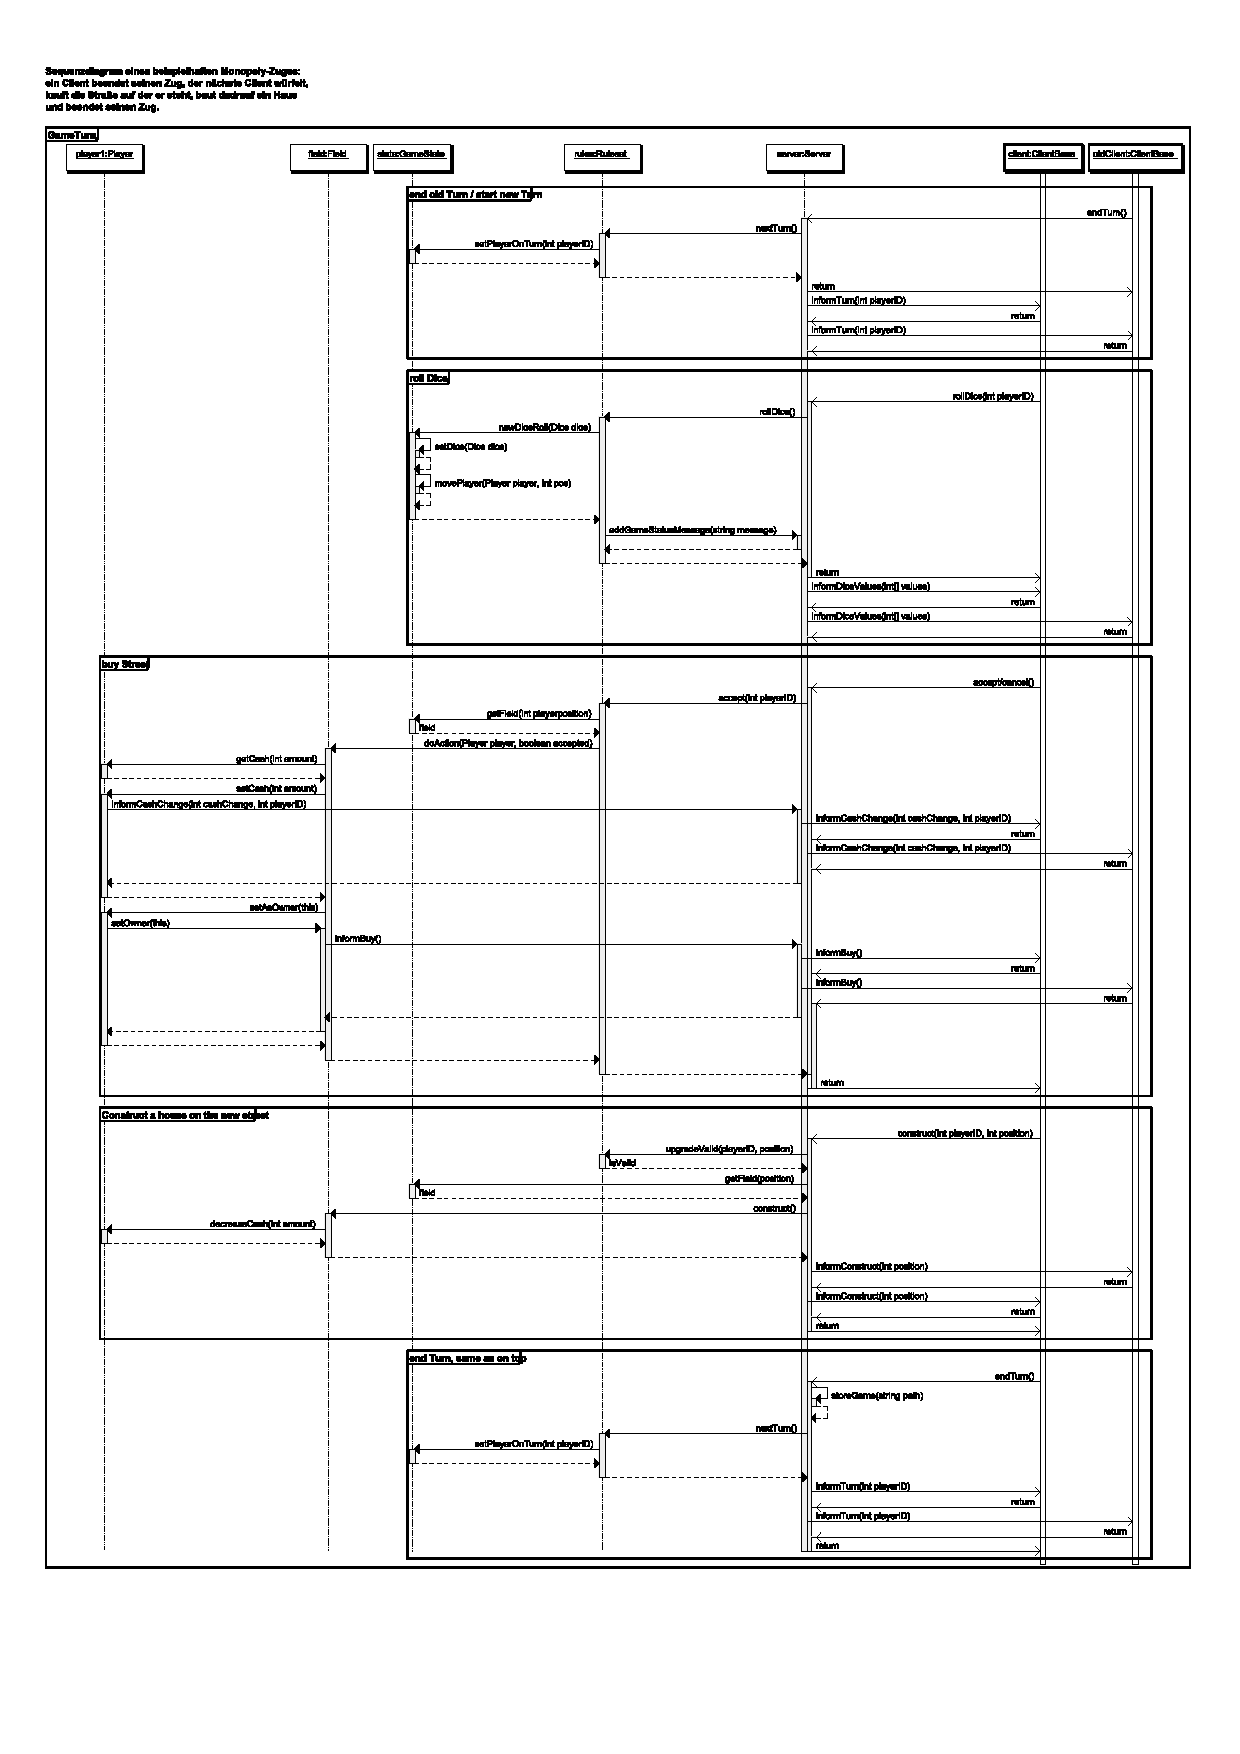
\includegraphics[width=18cm]{Sequenzdiagramme/Spielzug}
\newpage
\subsection{Verbinden eines Client auf einen Server}
Sobald ein Client sich auf einen (laufenden) Server verbinden will, müssen folgende Schritte stattfinden
\begin{enumerate}
\item Der (menschliche) Spieler gibt die IP-Addresse über ein Textfeld ein, der AIClient bekommt diese als Argument beim Starten übergeben
\item Der Client wird entweder direkt dem Server hinzugefügt (ein IClient-Objekt wird dem Server übergeben und ein IServer-Objekt dem Clienten) oder über das Netzwerk verbunden
\item Der Server fügt den Spieler seiner Spielerliste hinzu und initialisiert dessen Zustand
\end{enumerate}
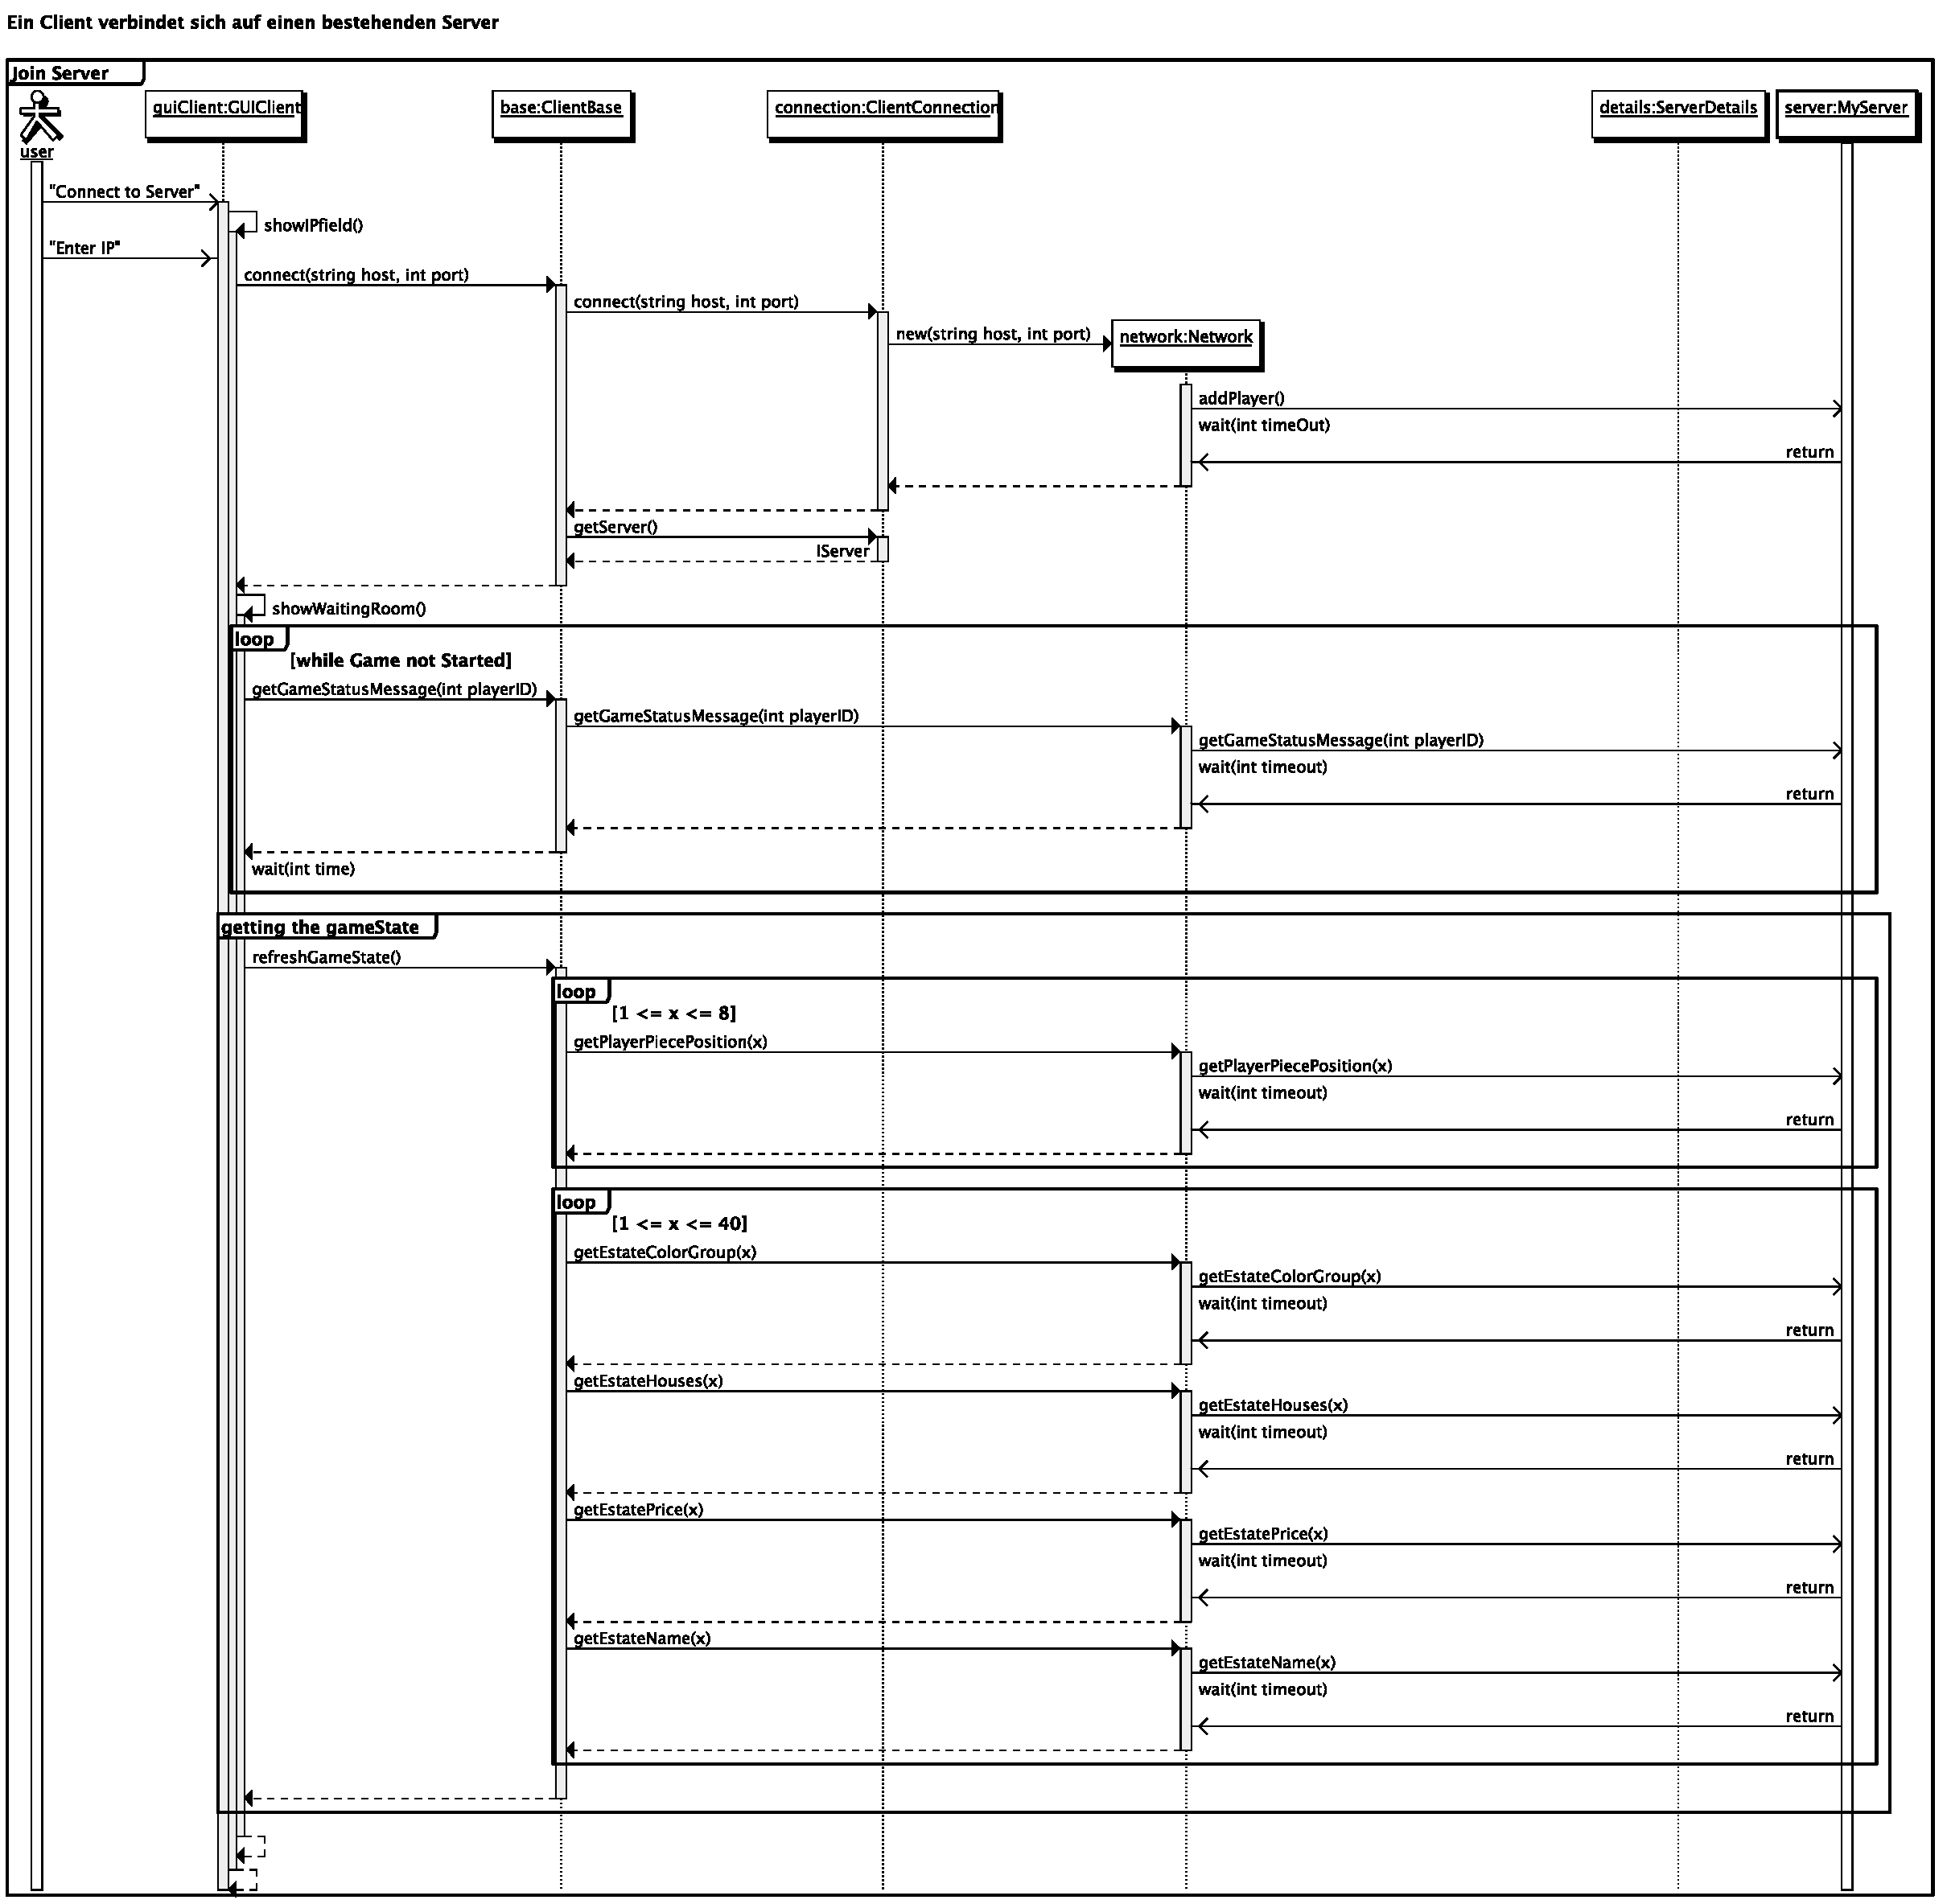
\includegraphics[width=17cm]{Sequenzdiagramme/client_verbinden}
\subsection{Beispielhafte Spielzüge}
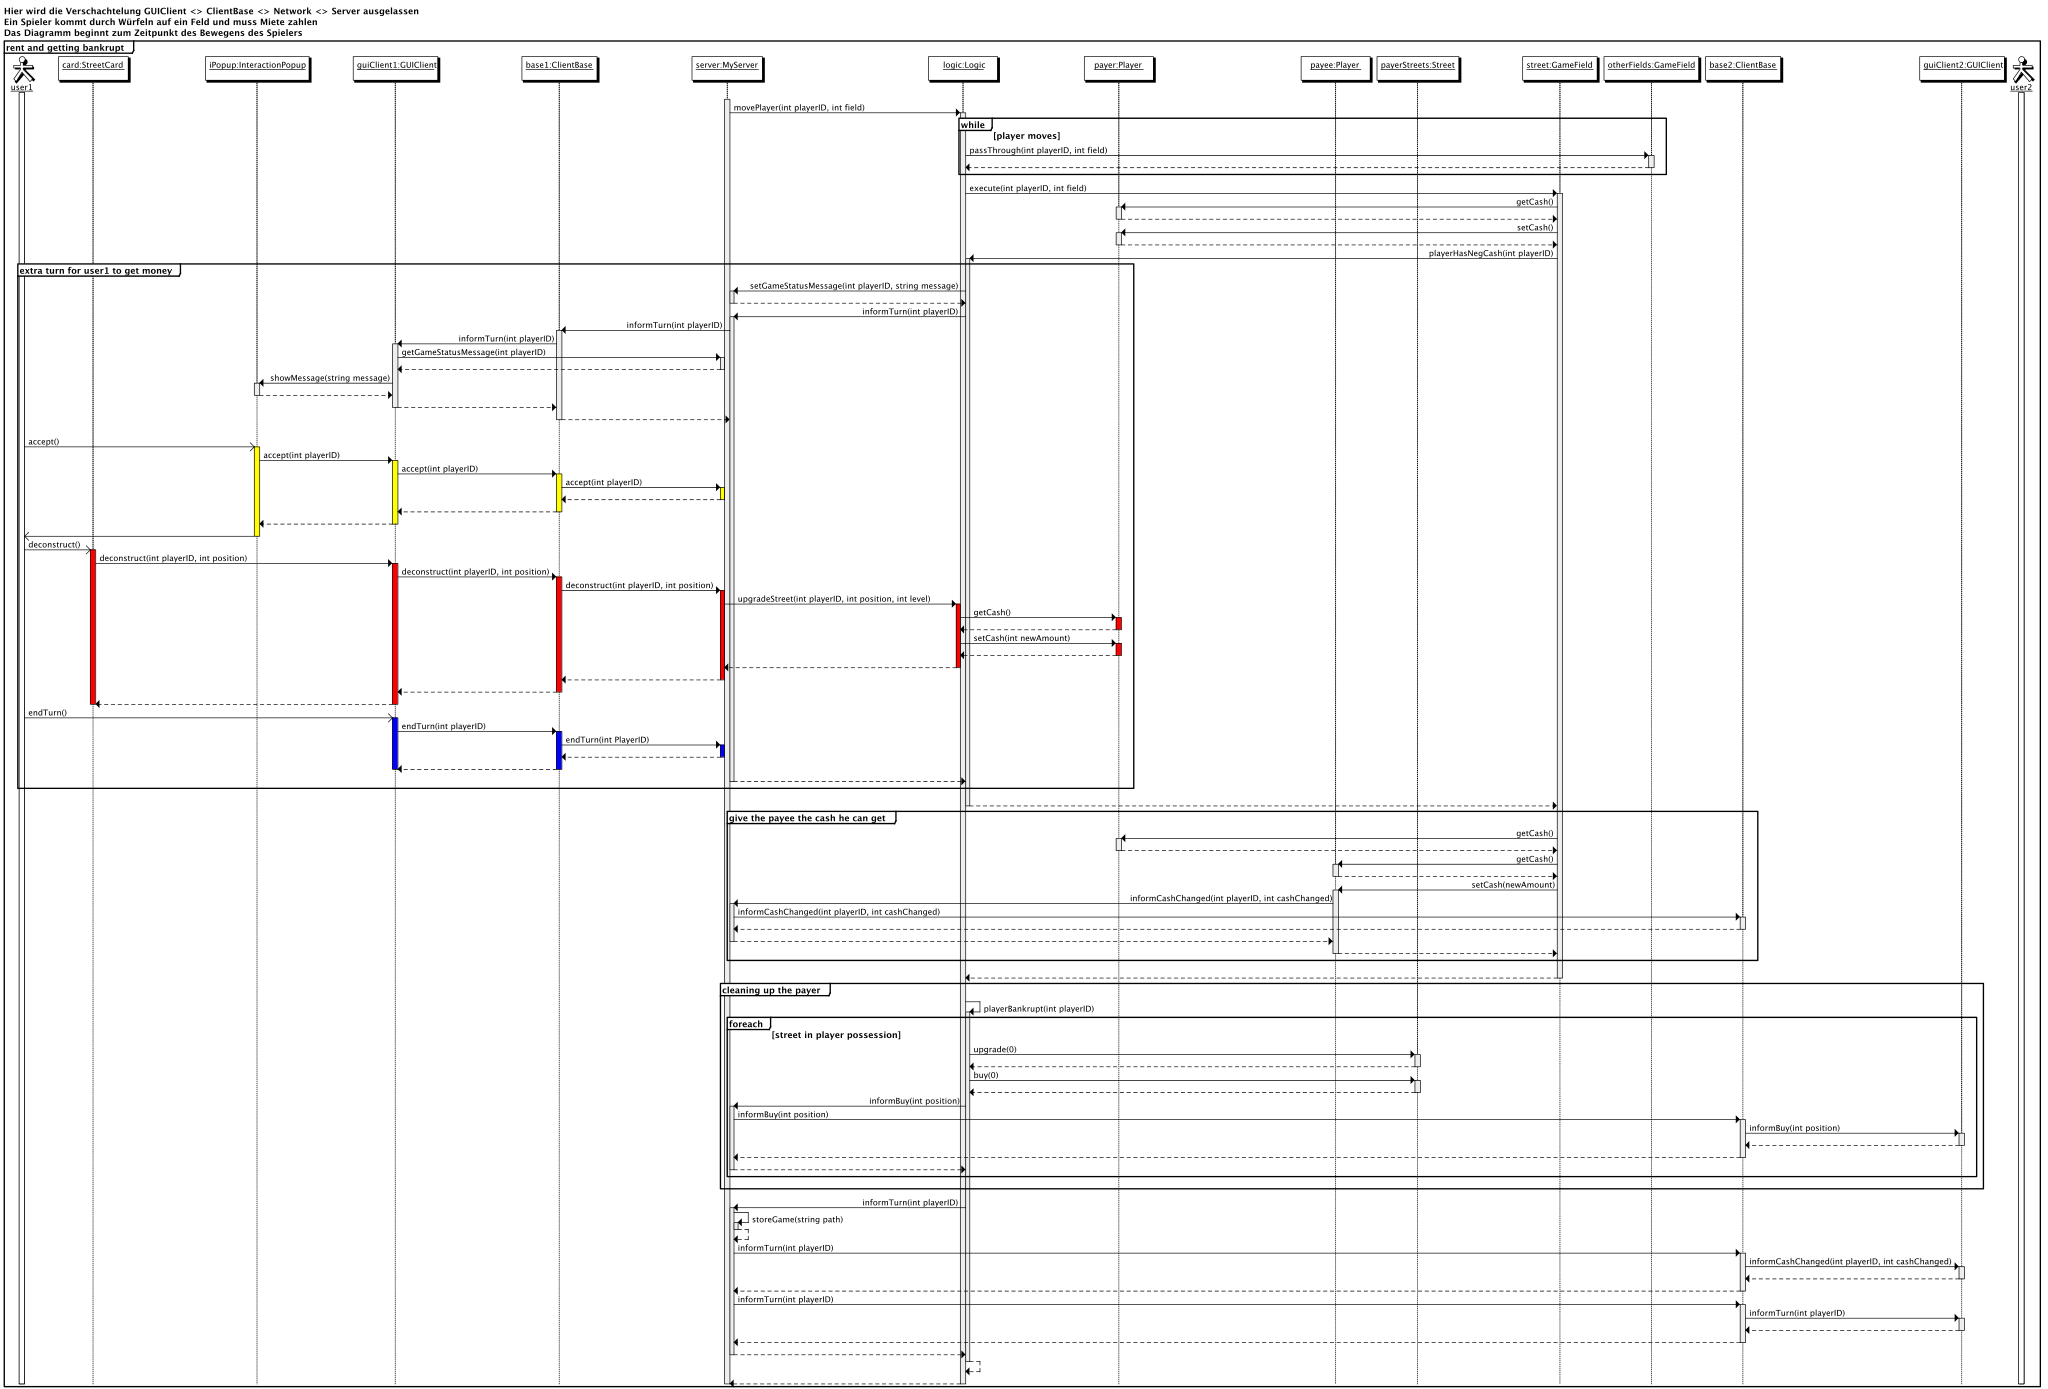
\includegraphics[angle = 90, height=23cm]{Sequenzdiagramme/bankrott_gehen}
\newpage
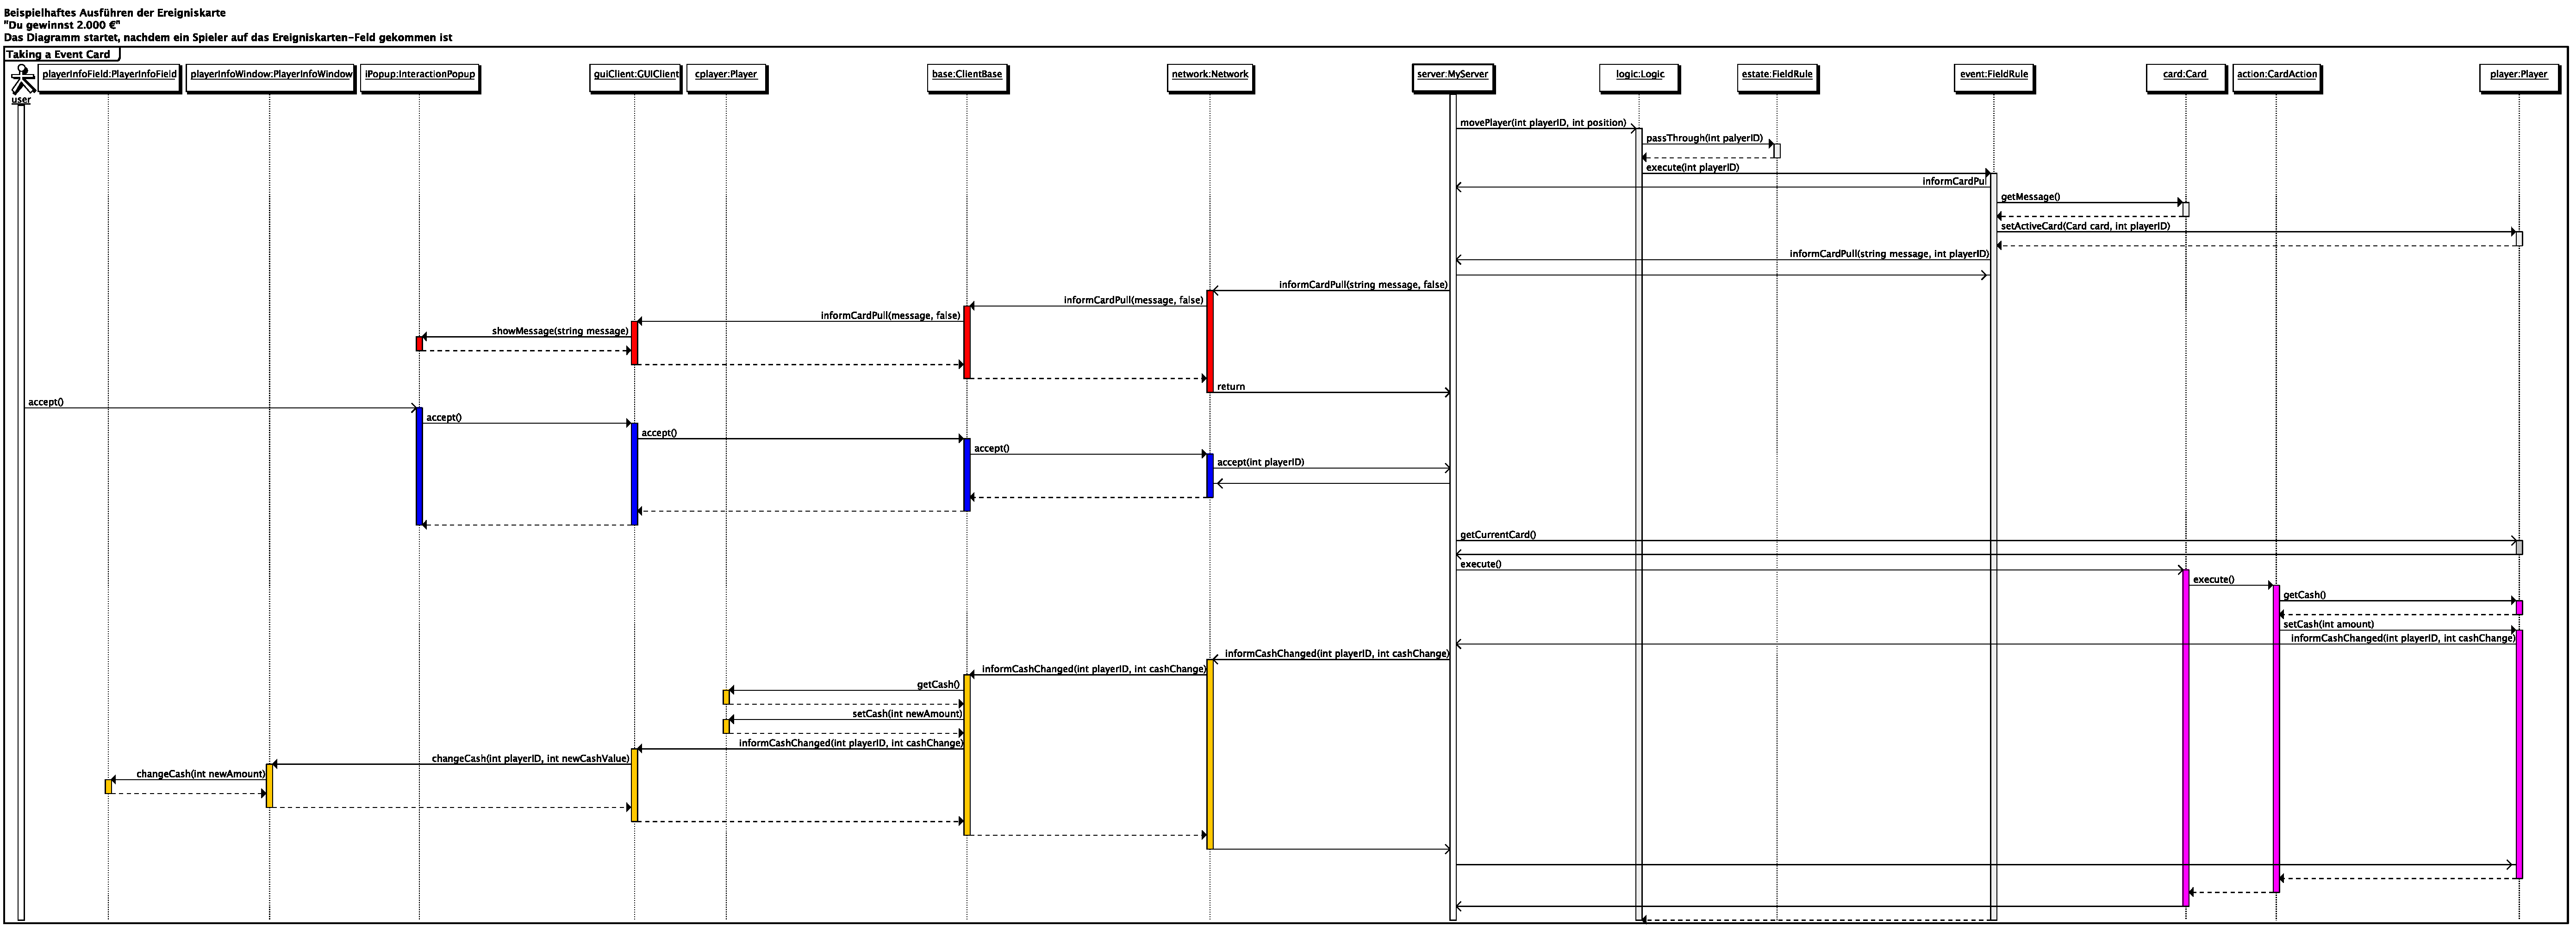
\includegraphics[angle = 90,height=24cm]{Sequenzdiagramme/Ereigniskarte}


\subsection{KI-Client-Zug}
Grundsätzlich baut der KI-Client auf der gleichen Klasse (\textit{ClientBase}) wie die "`normalen"' Clients auf. Von daher kann alles, was nicht für den KI-Client spezifisch ist, unter dem Punkt "`Durchführen eines Spielzugs"' nachgelesen werden. Es wird hier nur auf die Abweichungen eingegangen.

Die Arbeitsweise des KI-Clients orientiert sich an dem Paper von \textit{Frayn} und der Vorlesung zu dem Thema. Es stehen sechs einzelne Berwertungsfunktionen zur Verfügung (siehe Klassendiagramm), die von einer Gesamt-Bewertungsfunktion aufgerufen und gewichtet werden. Der Ablauf eines Zuges sieht folgendermaßen aus:
\begin{enumerate}
\item Aufrufen der \textit{returnBestCommand}-Methode von \textit{valuator}
\item Dieser überprüft anhand des übergebenen 
\item Übergeben jedes möglichen Spielzug an die Gesamt-Bewertungsfunktion. Diese ruft (falls passend) die einzelnen Bewertungsfunktionen auf, die abhängig vom aktuellen Spielzustand den möglichen Zug bewerten. Von allen möglichen Zügen wird derjenige mit der besten Bewertung ausgeführt.
\end{enumerate}
Beispiel-Zug:\\
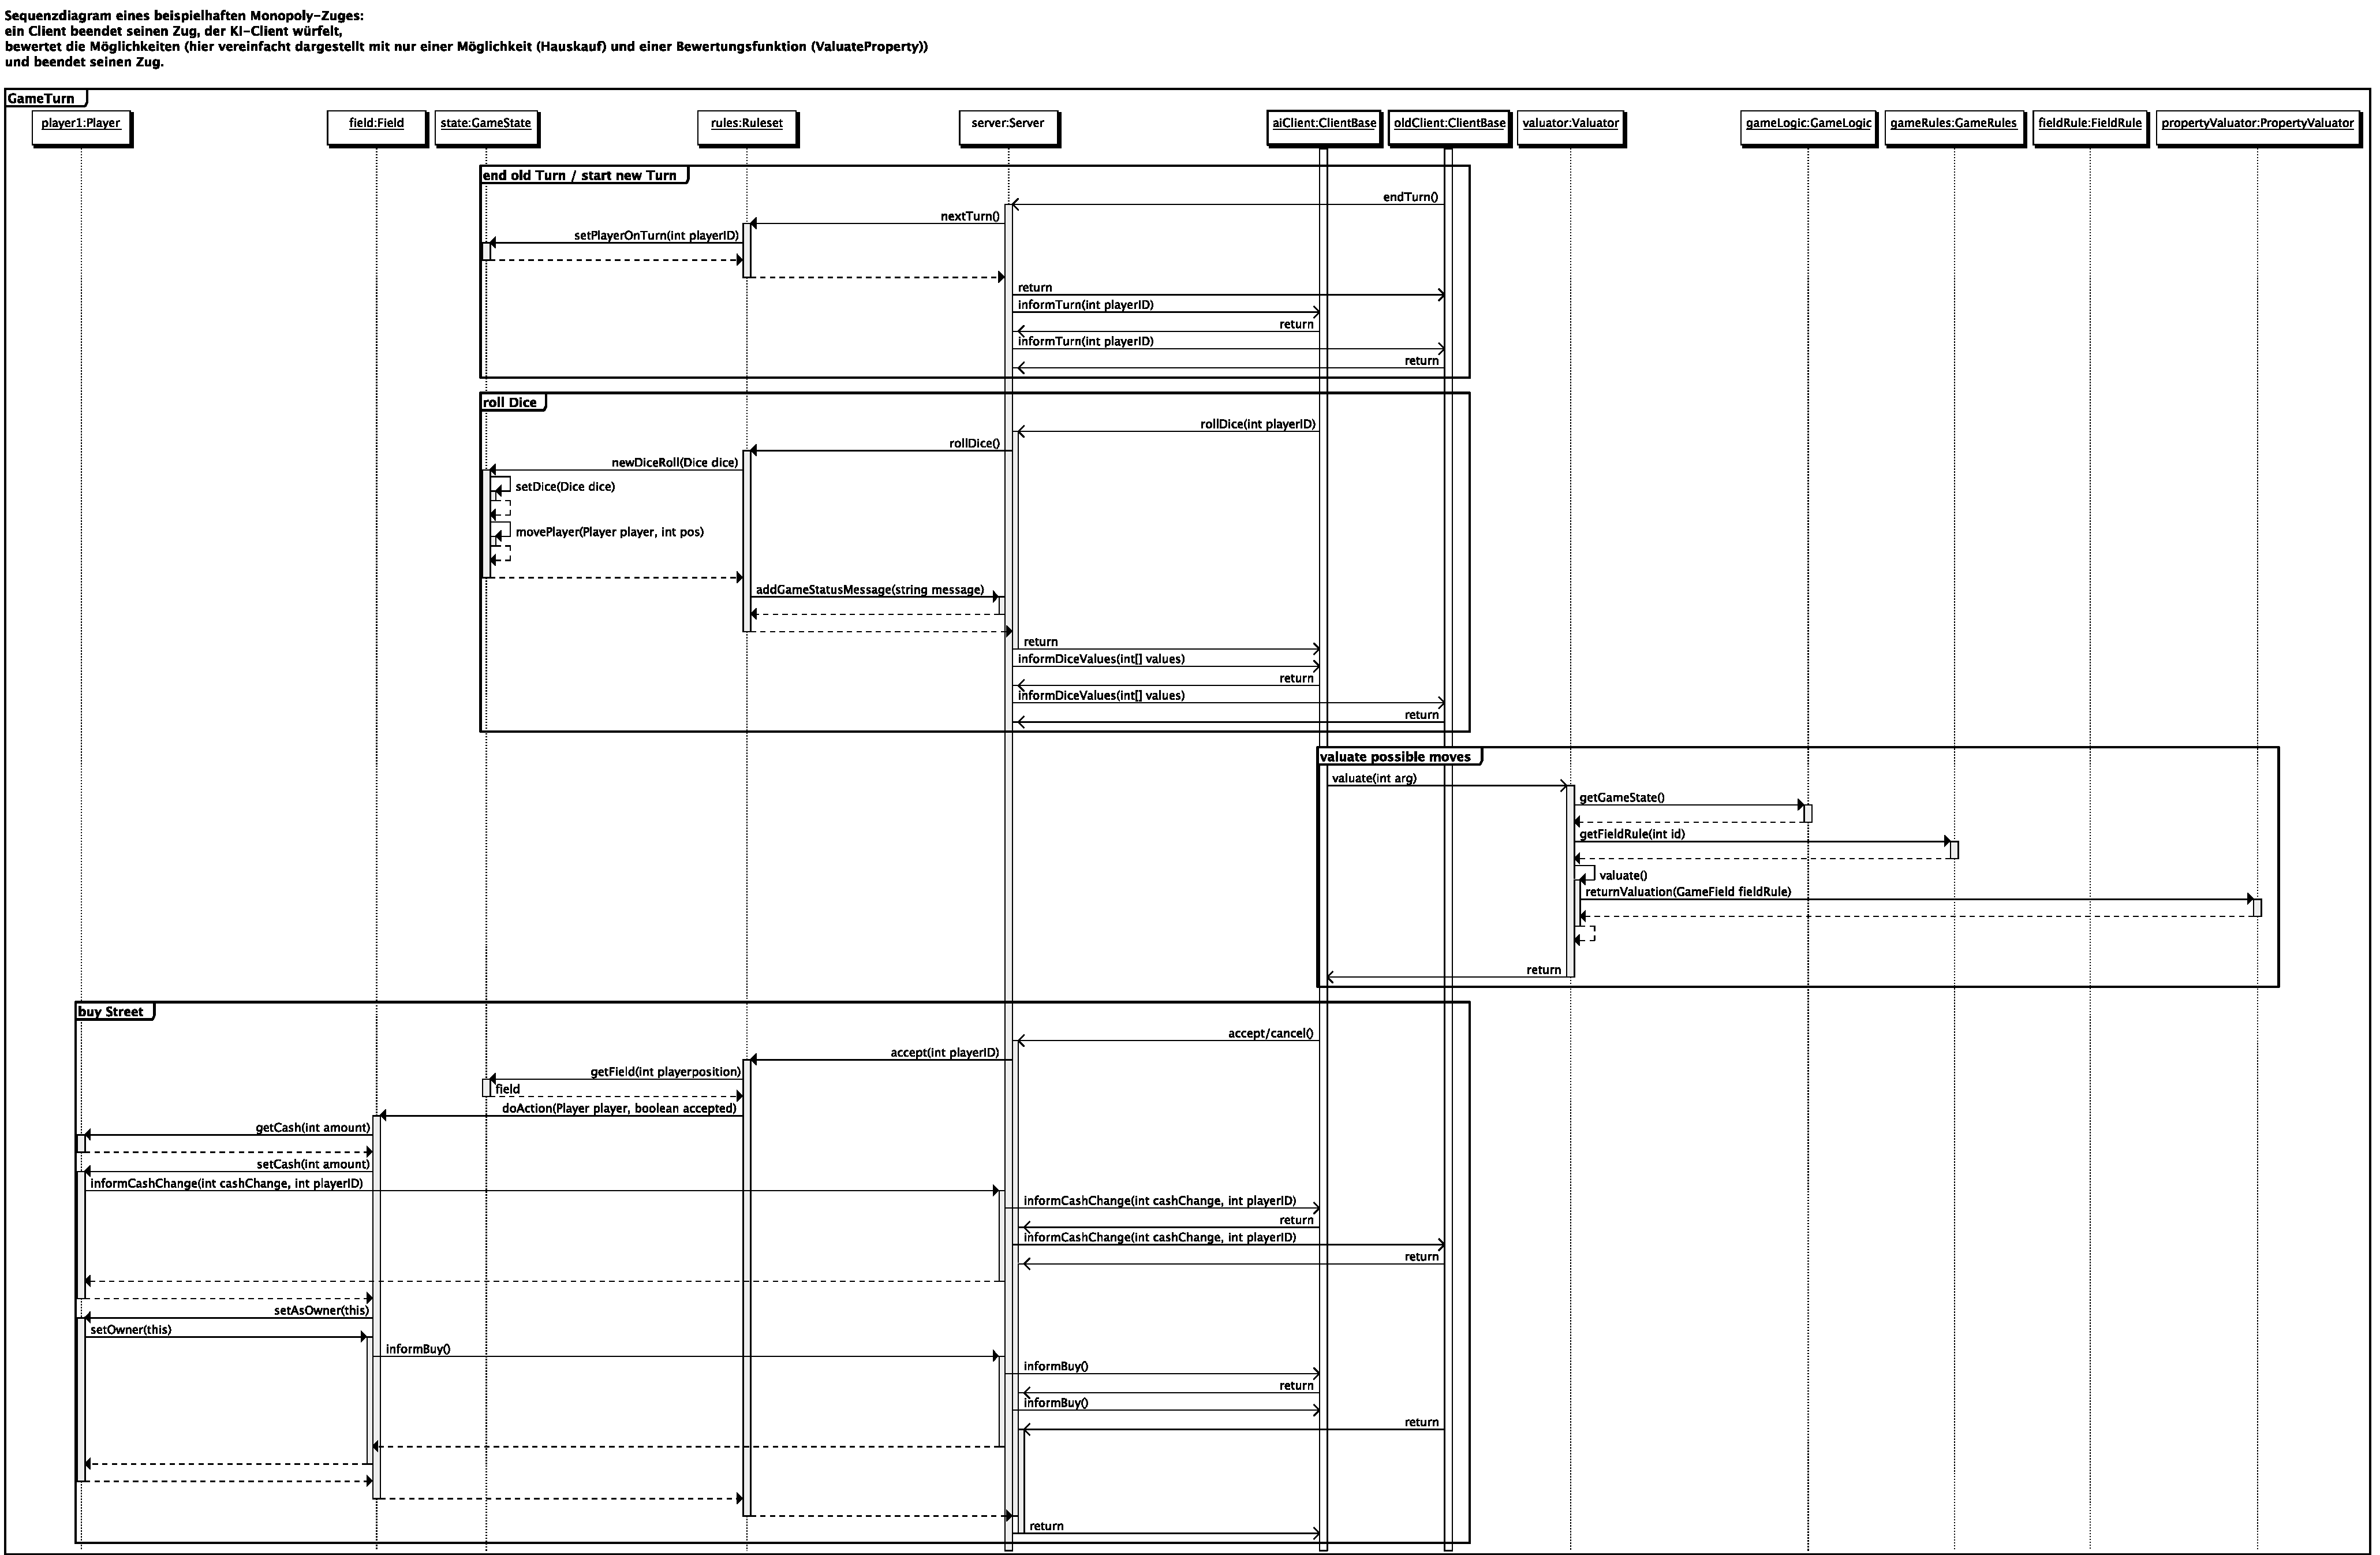
\includegraphics[angle = 90,height=17cm]{Sequenzdiagramme/ki_spielzug}
\section{Weitere Entwurfdetails}
\subsection{Kompatibilität mit Client und Server der anderen Gruppe}
Während der Entwurfsphase fanden mehrere Treffen mit einem Verantwortlichen der anderen Gruppe statt. Im Vorfeld wurde versucht, Punkte, an denen es Missverständnisse geben könnte, zu identifizieren. Im Zuge dessen wurden die vorgegebenen Interfaces erweitert und verändert, ein eigenes Interface für den Client definiert. Obwohl beide Gruppen unterschiedliche Entwurfsansätze verfolgen, sollte zumindest nach jetzigem Kenntnisstand einer erfolgreichen Kommunikation nichts im Wege stehen. Beim Abstimmungsprozess wurden zugunsten der Kompatibilität Einschränkungen bei der Erweiterbarkeit hingenommen.
\section{Abweichungen vom Pflichtenheft}
% besserer Name?
\begin{itemize}
\item Im Pflichtenheft wurde beschrieben, dass der Server alle vom Client einkommenden Nachrichten/Befehle darauf "uberpr"uft, ob diese auch vom richtigen Clienten kommen, sodass es nicht m"oglich ist, sich als "falscher" Client auszugeben. Da dies allerdings nicht gefordert war/ist, wurde dies nicht modelliert. Da die Validierung als recht eigenst"andige Schicht zwischen Server-Netzwerkanschluss und Server-Spiellogik liegen sollte, ist es problemlos m"ogloch, diese zus"atzliche Schicht auszulassen. Das hei"st, dass sich abseits der Validierung keine "Anderungen an Architektur und Design ergeben.
\item Nach Besprechungen innerhalb unserer Gruppe und gemeinsam mit der anderen Gruppe wurde beschlossen, den Nachrichtenflu"s zwischen Clienten und Server so umzugestalten, dass der Server nun statt passiv Anfragen der Clients zu bearbeiten auch aktiv Benachrichtigungen an dieselben schickt. F"ur diesen Zweck wurde zusammen mit der anderen Gruppe die Schnittstelle \textit{IClient} konzipiert, die auf "ahnliche Weise wie \textit{IServer} funktionieren soll, d.h. die meisten Methoden der Schnittstelle \textit{IServer} haben ein entgegengesetztes "Aquivalent in der Schnittstelle \textit{IClient}
\item Da bei beiden Monopoly-Gruppen das Spiel lokalisierbar sein soll und trotzdem Bereiche des Spielbretts/Spielfelds variabel gestaltet werden sollen, werden Stra"sennamen und "ahnliches vom Server in lokalisierter Fassung bereitgestellt. Dies f"uhrt aber auch dazu, dass anders als im Pflichtenheft der Spielplan nicht beim Clienten abgespeichert wird, sondern beim Server. Am Anfang eines Spieles, oder bei Bedarf, besorgt sich der Client vom Server alle f"ur ihn relevanten Daten als lokalisierten Text.
\item Im Pflichtenheft wurde vorgesehen, dass auch die Clients den Spielstand speichern k"onnen. Da dies aber wegen m"oglicherweise inkonsistenten Zust"anden und mangelnder Kompatibilität viel Zusatzarbeit bedeuten w"urde, wurde darauf verzichtet. Der Spielzustand wird also nur vom Server vollst"andig gespeichert, Clients werden zwar "uber "Anderungen daran informiert, aber haben keinen Bedarf mehr daran, dies l"angerfristig zu speichern.
\item Im Pflichtenheft ist eine spielspezifische maximale Spieleranzahl nicht vorgesehen, aus Gr"unden der Einfachheit wurde diese aber eingef"uhrt. Ein Spiel startet nun, wenn sich die maximale Anzahl von Clienten im Wartezustand befinden. Dies f"uhrt zu einer Reduzierung des Warteraums, es ist dort nicht mehr m"oglich, sich selbst als "`Zum Spielen bereit"' zu setzen, was auch Probleme mit der Kompatibilit"at des Servers der anderen Gruppe verhindern sollte.
\item Ebenfalls verzichtet wurde auf die M"oglichkeit, ein Spiel aktiv aufzugeben und trotzdem weiterhin zuzuschauen.
\item Im Pflichtenheft war es nur vorgesehen, dass ein \textit{AIClient} von au"serhalb des Servers Zugriff auf das Spiel hat. Das hei"st, dass ein \textit{AIClient} als eigenes Programm gestartet werdenund sich dann auf den Server verbinden müsste. Es ist nun aber auch m"oglich, direkt vom Server aus einen solchen Clienten dem Spiel hinzuzuf"ugen.
\item Es ist nicht möglich, einem angefangenen Spiel (wieder) beizutreten
\item /F11160/ "`Spielstand laden"' und /F11170/ "`Spielstand speichern"' wurden fallengelassen 
\end{itemize}
\section{Verantwortlichkeiten und weitere Planungen}
Die Leitung der einzelnen Abschnitte wird von folgenden Personen übernommen und vorgestellt:
\begin{description}
% Nennen?
\item[Pflichtenheft] Philip Caroli
% Nennen?
\item[Entwurf] Fabian Neundorf
\item[Implementierung] Jeremias Mechler
\item[Validierung] Usman Ghani Ahmed
\item[Präsentation] Maximilian Madlung
\end{description}
Zusätzlich übernimmt Fabian Neundorf die Kommunikation mit der anderen Gruppe und stimmt sich mit den Verantwortlichen ab.

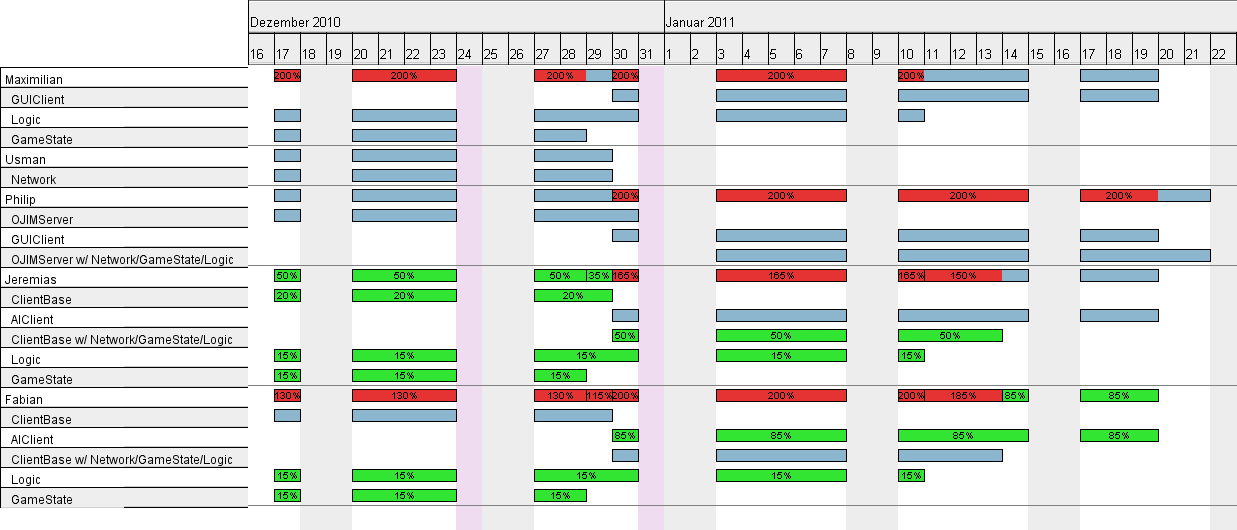
\includegraphics[width=17cm]{Gantt/gantt2}
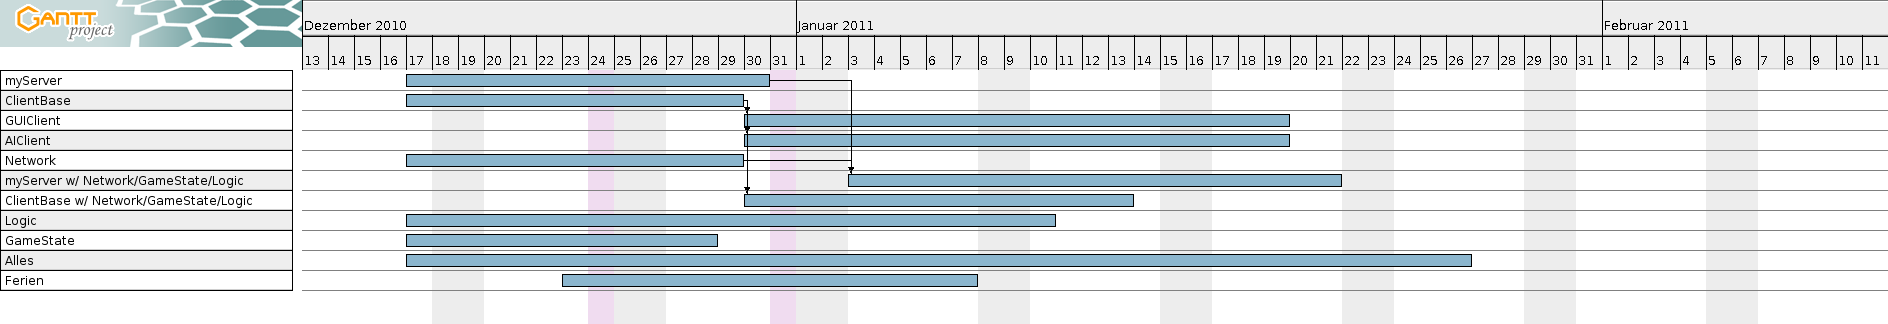
\includegraphics[width=17cm]{Gantt/gantt}
\section{Klassendiagramm}
Das Klassendiagramm befindet sich als \textit{pdf}-Datei in "`class\_diagram.pdf"'.
\section{Weitere Informationen}
Ein Teil der Beschreibungen der Methoden aus \textit{IServer, IServerTrade} und \textit{IServerAuction} stammen von Daniel Bruns.
\section{Änderungen zwischen Version 1.0 und 1.1}
\end{document}
